\chapter{Probabilistic SED Fitting Algorithm} \label{chp:Algorithm}
\captionsetup{width=0.75\textwidth}


The central theme is that probability calculus is the unique language within which we can develop models of our surroundings that have predictive capability. Probability calculus is uniquely defined\cite{Skilling2005} as the preferred language of inference.
The SED fitting technique implemented in the present thesis is established on Bayesian statistics.


%---------------------------------------------------------------------------%
%---------------------------------------------------------------------------%
%---------------------------------------------------------------------------%

\section{Bayesian Framework}\label{sec:Bayes}

In Bayesian statistics, the knowledge concerning the relative probability of various parametre values $\mathbf{\Theta}$ under the hypothesis $\mathcal{H}$ in the absence of any data is encoded in the prior probability density distribution $\mathscr{P}_{\mbox{prior}}(\mathbf{\Theta}| \mathcal{H})$ on the space of all possible parametres $\mathbf{\Theta}$. 
The probability of a particular value of $\mathbf{\Theta}$ given a specific data set $D$ under hypothesis $\mathcal{H}$ is written as a posterior probability density function (according to Bayes’ theorem) as: 
\begin{equation}
    \mathscr{P}_{\mbox{posterior}}(\mathbf{\Theta}|D, \mathcal{H}) = \dfrac{\mathscr{P}_{\mbox{prior}}(\mathbf{\Theta}|\mathcal{H})\,\mathscr{L}(D|\mathbf{\Theta}, \mathcal{H})}{\mathscr{E}(D|\mathcal{H}) } \label{eq:Bayes}
\end{equation}
where $\mathscr{L}(D|\mathbf{\Theta}, \mathcal{H} )$ the probability of obtaining the new data under the assumption of a certain set of parametre values, and it is called the likelihood. The Bayesian evidence, or marginal likelihood $\mathscr{E}(D| \mathcal{H})$ is the probability of the hypothesis explaining the data. The hypothesis consists of the SED model parameterisation that encompasses the model components discussed in Chapter \ref{chp:SED}.
The posterior probability density function can be used to obtain a best estimate and credibility interval for any model property $Y(\mathbf{\Theta})$.
The probability of the derived parameter $Y(\mathbf{\Theta})$ given the data is then
\begin{equation}
    \mathscr{P}_{posterior}(Y|D) \,dY = \int_Y \, \mathscr{P}_{posterior}(\mathbf{\Theta}|D) \,d\mathbf{\Theta} 
\end{equation}
where the integral extends over all $\mathbf\Theta$ for which $Y$ lies in a specified bin $\pm dY/2$. The most probable value of $Y$ can then be taken as the peak of this distribution and the most typical value as its median. The 95 per cent (symmetric) credibility interval of the distribution for scalar $Y$ can be defined and yields the uncertainty. The parametre investigated in the present work is the total stellar mass of each galaxy, in order to construct the stellar mass function.
More details regarding Bayesian methods can be found on Appendix \ref{app:Bayes}.

%the prior is taken to be the distribution of possible star formation histories in the comparison library, which can be viewed as a Monte Carlo sampling of f p (P). The integral in the above expression for the likelihood of Y is then trivially evaluated through binning the integrand as a function of Y. 

\section{Parametre Space, Likelihood \textit{\&} Priors}
The parametre space describing the total galaxy emission is 21-dimensional, as given by the number of parameters listed in Table \ref{tab:ParamSpace}. It is composed by two different types of parametres: shape parameters, which determine the shape of the templates and hence represent non-linear dependencies, and amplitude parameters, on which the model depends linearly and which scale the contribution strength of each component. The ranges that we assume for each parametre are listed in the fourth column of Table \ref{tab:ParamSpace}. \\
As discussed in Section \ref{sec:SED/AGNtorus}, the parametres shaping the AGN torus models are
\begin{equation}
    \vec{\theta}_{\mbox{\tiny{AGN}}} = (i_{\mbox{\tiny{view}}}, \theta_{\mbox{\tiny{clouds}}} , N_{\mbox{\tiny{0,AGN}}}, \alpha_{\mbox{\tiny{AGN}}} )
\end{equation}
Since the AGN torus component's physical parametres and morphology are not the central research theme of the present thesis, and none of them is coupled to any prior in this work's model implementation, although the algorithm fits them as well as every other parametre, for demonstration purposes they will be represented by the notion  $\vec{\theta}_{\mbox{\tiny{AGN}}}$.
The inclination angle $i_{\mbox{\tiny{view}}}$ has a range of [$0^o, 90^o$], the half angle mapping the torus from the equatorial plane has a range of [$14^o, 51^o$], the number of clouds in the equatorial line of sight $N_{\mbox{\tiny{0,AGN}}}$ has a range of [5,10] and the spectral index $ \alpha_{\mbox{\tiny{AGN}}}$ has a range of [-2.25, -0.25]. To each of those shaping parametres of the AGN model corresponds a uniform prior at the respective range. \\
As shown in Table \ref{tab:ParamSpace}, two composite stellar population models of delayed exponential decay SFH are used, differing in age, so that a more complex SFH function could be modeled. Hereby called Old Stellar Population and Young Stellar Population, the Old Stellar Population models a delayed exponential decay SFH that started between the Big Bang (age of the universe at galaxy's redshift) and 1 Gyr ago and the Young Stellar Population models a delayed exponential decay SFH that started between 1 Gyr and 1Myr ago. The Stellar Mass of both stellar populations is fit and both are taken into account for the inference of galaxy stellar mass. 
\begin{table}
\caption{Parametres used for modelling the ARC SEDs. The parametre and its description are in the second and third columns, respectively. The galaxy component to which they appertain is listed in the first column, the range of values and the shape of the prior distribution are listed in the fourth and fifth column.}
    \centering
    \begin{tabular}{ccccc}
    \addlinespace
    \hline  %\toprule
    Component & Parametre & Description & Range &  Prior      \\
    \hline   %\midrule
    \hline   %\midrule
    %---------------------------------------------% 
    \multirow{5}{4em}{Old Stars} & $ M_\star/M_\odot$ & Stellar Mass & [$10^7$,$10^{15}$] & logUniform \\ 
                                & $Z_\star/Z_\odot$ &  Metallicity & [0, 5] & Uniform \\ 
                                & $t/$Myrs & age of CSP & [1000,Age of Universe at z] & logUniform \\ 
                                & $\tau/$Gyrs & Stellar Metallicity & [0.01, 14] & logUniform \\ 
                                & E(B-V) & color excess & [0,1] & Uniform \\          
    \hline
    \multirow{5}{4em}{Young Stars} & $ M_\star/M_\odot$ & Stellar Mass & [$10^7$,$10^{15}$] & logUniform \\ 
                                & $Z_\star/Z_\odot$ &  Metallicity & [0, 5] & Uniform \\ 
                                & $t/$Myrs & age of CSP & [1,1000] & logUniform \\ 
                                & $\tau/$Gyrs & Stellar Metallicity & [0.01, 14] & logUniform \\ 
                                & E(B-V) & color excess & [0,1] & Uniform \\
    \hline
    \multirow{2}{4em}{ISM dust } & $ M_{\mbox{\tiny{dust}}}/M_\odot$ & dust Mass & [$10^0$,$10^{20}$] & logUniform \\ 
                                & $\alpha_{\mbox{\tiny{SF}}}$ &  dust index & [0, 4.5] & Uniform \\ 
    \hline
    \multirow{2}{4em}{BBB } &  $A_{\mbox{\tiny{BBB}}}$ &  BBB amplitude & [$10^{-10}$,$10^5$] & logUniform \\ 
                            & E(B-V)$_{\mbox{\tiny{BBB}}}$ & reddening & [0,1] & Uniform \\ 
    \hline
    \multirow{2}{4em}{AGN torus } & $A_{\mbox{\tiny{AGN}}}$ & AGN amplitude & [$10^{-10}$,$10^8$] & logUniform \\ 
                                & $\vec{\theta}_{\mbox{\tiny{AGN}}} $ &  shape parametres & full range & Uniforms \\ 
    \hline
    \multirow{2}{4em}{radio } & $A_{\mbox{\tiny{radio}}}$ & synchrotron amplitude & [$10^{13}$,$10^{60}$] & logUniform \\ 
                                & $\alpha_{\mbox{\tiny{radio}}}$ &  spectral index & [-3, 3] & Uniform \\ 
    \hline
    \hline
    \end{tabular}  
    \label{tab:ParamSpace}
\end{table}
%---------------------------------------------------------------------------%
\subsection{Likelihood}\label{sec:Likeli}

The basic ln-likelihood calculation is effectively a χ$^2$ calculation for the photometric data. This gives the following expression for the ln-likelihood:
\begin{equation*} 
\begin{aligned}
\mathscr{L}(D|\Theta)  & = \mathscr{L}_{\mbox{\tiny{old stellar}}}(D| Z_{\mbox{\tiny{o}}}, t_{\mbox{\tiny{o}}}, \tau_{\mbox{\tiny{o}}}, \log M_{\star, \mbox{\tiny{o}}}, EBV_{\mbox{\tiny{o}}})  \times  \mathscr{L}_{\mbox{\tiny{young stellar}}}(D| Z_{\mbox{\tiny{y}}}, t_{\mbox{\tiny{y}}}, \tau_{\mbox{\tiny{y}}}, \log M_{\star, \mbox{\tiny{y}}}, EBV_{\mbox{\tiny{y}}}) \times \\  
& \times \mathscr{L}_{\mbox{\tiny{ISM dust}}}(D|\alpha_{\mbox{\tiny{SF}}}, \log M_{\mbox{\tiny{dust}}})  \times  \mathscr{L}_{\mbox{\tiny{BBB}}}(D|A_{\mbox{\tiny{BBB}}}, EBV_{\mbox{\tiny{BBB}}}) \times  \mathscr{L}_{\mbox{\tiny{radio}}}(D|A_{\mbox{\tiny{radio}}}, \alpha_{\mbox{\tiny{radio}}}) \times   \\ 
& \times\mathscr{L}_{\mbox{\tiny{AGN torus}}}(D|A_{\mbox{\tiny{AGN}}}, \vec{\theta}_{\mbox{\tiny{AGN}}})   \iff 
\end{aligned} 
\end{equation*}
\begin{equation} 
\begin{aligned}
\iff \ln \mathscr{L}(D|\Theta)  & =\ln \mathscr{L}_{\mbox{\tiny{old stellar}}}(D| Z_{\mbox{\tiny{o}}}, t_{\mbox{\tiny{o}}}, \tau_{\mbox{\tiny{o}}}, \log M_{\star, \mbox{\tiny{o}}}, EBV_{\mbox{\tiny{o}}})  + \\
&+\ln \mathscr{L}_{\mbox{\tiny{young stellar}}}(D| Z_{\mbox{\tiny{y}}}, t_{\mbox{\tiny{y}}}, \tau_{\mbox{\tiny{y}}}, \log M_{\star, \mbox{\tiny{y}}}, EBV_{\mbox{\tiny{y}}}) + \\  
& +\ln \mathscr{L}_{\mbox{\tiny{ISM dust}}}(D|\alpha_{\mbox{\tiny{SF}}}, \log M_{\mbox{\tiny{dust}}})  +  \ln \mathscr{L}_{\mbox{\tiny{BBB}}}(D|A_{\mbox{\tiny{BBB}}}, EBV_{\mbox{\tiny{BBB}}}) + \\
& +\ln \mathscr{L}_{\mbox{\tiny{radio}}}(D|A_{\mbox{\tiny{radio}}}, \alpha_{\mbox{\tiny{radio}}}) +   \ln \mathscr{L}_{\mbox{\tiny{AGN torus}}}(D|A_{\mbox{\tiny{AGN}}}, \vec{\theta}_{\mbox{\tiny{AGN}}})  
\end{aligned} \label{eq:LikeliTot}
\end{equation}
The Likelihood function for each component are:
\begin{equation} \begin{split}
    \mathscr{L}&_{\mbox{\tiny{old stellar}}}(D| Z_{\mbox{\tiny{o}}}, t_{\mbox{\tiny{o}}}, \tau_{\mbox{\tiny{o}}}, \log M_{\star, \mbox{\tiny{o}}}, EBV_{\mbox{\tiny{o}}}) = \\ & =  \dfrac{1}{\sigma_i\sqrt{2\pi} }  \mbox{exp} \sum_{i=1}^{N}\; \dfrac{ \Big[ \mbox{ModelSEDphot}_i\Big( Z_{\mbox{\tiny{o}}}, t_{\mbox{\tiny{o}}}, \tau_{\mbox{\tiny{o}}}, \log M_{\star, \mbox{\tiny{o}}}, EBV_{\mbox{\tiny{o}}}\Big)- \mbox{ObsPhot}_i   \Big]^2}{ 2 \sigma_i^2   }
  \end{split} \label{eq:LikeliOS}
\end{equation} 
\begin{equation} \begin{split}
    \mathscr{L}&_{\mbox{\tiny{young stellar}}}(D| Z_{\mbox{\tiny{y}}}, t_{\mbox{\tiny{y}}}, \tau_{\mbox{\tiny{y}}}, \log M_{\star, \mbox{\tiny{y}}}, EBV_{\mbox{\tiny{y}}})   = \\ & =  \dfrac{1}{\sigma_i\sqrt{2\pi} }\mbox{exp} \sum_{i=1}^{N}\; \dfrac{ \Big[ \mbox{ModelSEDphot}_i\Big( Z_{\mbox{\tiny{y}}}, t_{\mbox{\tiny{y}}}, \tau_{\mbox{\tiny{y}}}, \log M_{\star, \mbox{\tiny{y}}}, EBV_{\mbox{\tiny{y}}}\Big)- \mbox{ObsPhot}_i   \Big]^2}{ 2 \sigma_i^2   }
  \end{split} \label{eq:LikeliYS}
\end{equation} 
\begin{equation}\begin{split}
   \mathscr{L}_{\mbox{\tiny{ISM dust}}}&(D|\alpha_{\mbox{\tiny{SF}}}, \log M_{\mbox{\tiny{dust}}}) = \\ & = \dfrac{1}{\sigma_i\sqrt{2\pi} } \mbox{exp} \sum_{i=1}^{N}\; \dfrac{ \Big[ \mbox{ModelSEDphot}_i\Big( \alpha_{\mbox{\tiny{SF}}}, \log M_{\mbox{\tiny{dust}}}\Big)- \mbox{ObsPhot}_i   \Big]^2}{ 2 \sigma_i^2   }  \end{split}  \label{eq:LikeliDust}
\end{equation}
\begin{equation} \begin{split}
   \mathscr{L}_{\mbox{\tiny{BBB}}}&(D|A_{\mbox{\tiny{BBB}}}, EBV_{\mbox{\tiny{BBB}}}) = \\ & = \dfrac{1}{\sigma_i\sqrt{2\pi} }\mbox{exp} \sum_{i=1}^{N}\; \dfrac{ \Big[ \mbox{ModelSEDphot}_i\Big( A_{\mbox{\tiny{BBB}}}, EBV_{\mbox{\tiny{BBB}}}\Big)- \mbox{ObsPhot}_i   \Big]^2}{ 2 \sigma_i^2   } \end{split}  \label{eq:LikeliBBB}
 \end{equation}
\begin{equation}\begin{split} 
 \mathscr{L}_{\mbox{\tiny{AGN torus}}}&(D|A_{\mbox{\tiny{AGN}}}, \vec{\theta}_{\mbox{\tiny{AGN}}})=\\ & =  \mbox{exp} \sum_{i=1}^{N}\; \dfrac{ \Big[ \mbox{ModelSEDphot}_i\Big( A_{\mbox{\tiny{AGN}}}, \vec{\theta}_{\mbox{\tiny{AGN}}}\Big)- \mbox{ObsPhot}_i   \Big]^2}{ 2 \sigma_i^2   }  \end{split}   \label{eq:LikeliTor}
 \end{equation}
\begin{equation} \begin{split}
\mathscr{L}_{\mbox{\tiny{radio}}}&(D|A_{\mbox{\tiny{radio}}}, \alpha_{\mbox{\tiny{radio}}}) =\\ & =  \mbox{exp} \sum_{i=1}^{N}\; \dfrac{ \Big[ \mbox{ModelSEDphot}_i\Big( A_{\mbox{\tiny{radio}}}, \alpha_{\mbox{\tiny{radio}}} \Big)- \mbox{ObsPhot}_i   \Big]^2}{ 2 \sigma_i^2   } \end{split}    \label{eq:LikeliRad}
 \end{equation}
Where $i$ counts the SED data points, $N$ is the total number of SED data points (observations), $\mbox{ModelSEDphot}$ is the modelled SED for each component as described in Chapter \ref{chp:SED}, $\mbox{ObsPhot}$ is the observed SED for each galaxy and $\sigma_i$ is the measurement uncertainty for each SED data point.\\ \\
By default, known and independent Gaussian flux uncertainties are assumed. Under this assumption, the ln-likelihood for the photometric terms is simply χ$^2$. More complex noise models can be applied in order to adjust a variety of instrumental artifacts or to allow for properties of the noise itself to be inferred, or for the presence of correlated noise to be modeled.
This can be accomplished through a flexible noise covariance matrix construction.
The ln-likelihood for the more complex noise model is
\begin{equation}
    \ln \mathscr{L}(D|\vec\Theta) =-\dfrac{1}{2} \Big[  n_i \,\mathbf{C}^{-1}_{ij}(\vec\gamma) \, n_j  + \ln\|2\pi \mathbf{C}(\vec\gamma) \| \Big]  
\end{equation}
where $\vec\Theta$ represents the total parametres of the SED model $n_i$ is the noise model, $\mathbf{C}$ is the correlation matrix (identity matrix in case of Gaussian noise, diagonal matrix in case of stationary noise) and $\vec\gamma$ are the parametres which model the noise:
\begin{equation}
     n_i  =  \mbox{ObsPhot}_i  - \mbox{ModelSEDphot}_i( \vec\Theta)
\end{equation}
%---------------------------------------------------------------------------%
\subsection{Priors}\label{sec:Prior}\label{sec:priors}

In Bayesian inference the prior model provides a valuable opportunity to incorporate astrophysical knowledge into the inferences. 
Every parametre specified in the construction of the full SED model, as described in Chapter \ref{chp:SED}, can be fit using the code. When fitting a parametre, a prior probability distribution is specified, consisting of an upper and lower limit on the parameter value, and a functional form for the prior probability density between these limits. As shown in Table \ref{tab:ParamSpace}, the priors used are Uniform or logarithmic Uniform priors. 
The parametres of the components synthesising the SED spectrum of a galaxy have a large dynamic range, thus, a uniform prior in log space is chosen for the parametres that span many orders of magnitude.\\
The conjugate prior to a Gaussian likelihood is the Dirichlet distribution, which mostly resembles the Uniform distribution, and since Gaussian likelihoods are used for every SED model component, a case can be made\cite{Betancourt2012} in favour of Dirichlet priors for computational efficiency. Although the work presented here has made use of the aforementioned priors in Table \ref{tab:ParamSpace}.

\subsubsection*{Conditions as non-linear priors}
In order to impose a condition based on astrophysical knowledge or an observational constraint it is possible in principle to specify joint priors on several parameters or achieve those conditions through parameter transformations. In the present work the energy balance of ISM dust absorption and re-emission or AGN dusty torus absorption and re-emission is imposed. Those conditions function as non-linear priors and can play a central role in determining the shape of the posterior probability distribution in the often highly degenerate space of SED modeling.\\
The BBB emission upper limit discussed in Section \ref{sec:DataClean} as a proxy of the AGN fraction of the ARC sources, is also a non linear prior that can be used in a version of the code, although it is not implemented for the runs presented in the present thesis, since a more scrutinous curation of the Hubble Space Telescope data and, cosequently, selection of accretion disk upper limits is due. 

%---------------------------------------------------------------------------%
%---------------------------------------------------------------------------%
%---------------------------------------------------------------------------%
\section{Sampling Method, Optimisation \textit{\&} Implementation}\label{sec:SamplingMethod}

The sampling method chosen is the dynamic nested sampling which allows for efficient exploration of higher-dimensional, multimodal and highly degenerate parameter spaces\cite{Skilling2006}.
This is invaluable in many circumstances relevant to spectral fitting, notably when dealing solely with broad band photometric observations, where the age-metallicity-dust degeneracy often leads to poorly constrained and highly degenerate parameter estimates, several widely spaced local minima in parameter space, any of which can trap traditional numerical functional minimisation routines or Markov Chain Monte Carlo (MCMC) methods.
%---------------------------------------------------------------------------%
\subsection{Dynamic Nested Sampling}

Nested sampling\cite{Skilling2006} is a Monte Carlo algorithm based on successive draws from the prior distribution at increasing values of the likelihood. It uses\cite{NestSam2021} the change in the effective prior volume of isolikelihood contours as a function of likelihood to estimate the Bayesian evidence ($\mathscr{E}$ in equation  \ref{eq:Bayes}). The successive draws (cornered "live points"), along with their associated weights, give a direct estimate of the density of states and can be used to estimate the posterior distribution of the parameters as a by-product.\\
Because of the way the prior volume is sampled, nested sampling is well suited to posteriors that are multimodal. Furthermore, no optimisation is required before sampling begins, and stopping criteria based on estimates of the remaining evidence can be defined.
Posterior samples from nested sampling approximate the true posterior for continuous and discontinuous functions, respectively\cite{NestSample_2016}. \\ \\
Dynamic Nested Sampling is a modification of the nested sampling algorithm by dynamically varying the number of live points in order to maximise the accuracy of a calculation for some number of posterior samples, subject to practical constraints. Compared to standard nested sampling, dynamic nested sampling is particularly effective for parameter estimation because standard nested sampling typically spends most of its computational effort iterating towards the posterior peak. This produces posterior samples with negligible weights which make little contribution to parameter estimation calculations. Dynamic nested sampling, also, significantly improves\cite{Higson2019} the accuracy of evidence calculations, and shows both evidence and parameter estimation can be improved simultaneously.

\subsection{Software \textit{\&} Optimal Sampling}

The sampling software used as the main tool of the SED fitting algorithm of the present thesis is the  \code{UltraNest}\footnote{\url{https://johannesbuchner.github.io/UltraNest/}} package, developed by Johannes Buchner (2021)\cite{ultranest2021} which uses the Nested Sampling algorithm MLFriends described in the work of Buchner (2016, 2019)\cite{NestSample_2016}\cite{NestSample_2019}. \\
The \code{UltraNest} code uses Reactive Nested Sampling, which is a generalisation of the Dynamic Nested Sampling that uses a tree structure for adding live points. The root of the tree represents the entire prior volume, and the branch nodes are samples from the entire prior. The tree formulation of Reactive Nested Sampling makes implementing error propagation and variable number of live points unambiguous. 

\subsubsection*{Slice Sampling}
For problems with high dimensionality or many degeneracies, the computational effiency is low. This can be overcome by using several types of Monte Carlo random walks supported by the \code{UltraNest} software.
Nested Sampling with Slice Sampler\cite{Handley2015} utilises slice sampling at each iteration to sample within the hard likelihood constraint of nested sampling. It can identify and evolve separate modes of a posterior semi-independently. 

%---------------------------------------------------------------------------%
%---------------------------------------------------------------------------%
%---------------------------------------------------------------------------%
\section{Testing the Algorithm on Synthetic Data}


In order to ensure that the SED fitting procedure produces reliable results, extensive tests were performed. At first, each model component is tested, followed by generating a synthetic galaxy SED and fitting all components in aggregate.\\
The number of the \code{UltraNest} sampler live points in every run of this work is set to $800$. A finer sampling of parameter space can be achieved by increasing the number of live points to higher value (e.g. 3000 live points).  This will increase the reliability of the maximum likelihood values obtained, though the time to perform a fit will become longer.\\ \\
\subsection*{Individual Component Fits}
The Reactive Nested Sampling with Slice Sampler is benchmarked against the pure Reactive Nested Sampling as shown in Figure \ref{fig:ComponentPosterior}. The differences ar minimal, thus, the Reactive Nested Sampling with Slice Sampler is the chosen sampling method of the Bayesian SED fitting algorithm of this thesis, since it reduced the time for fitting an all-component SED model to an observed ARC galaxy SED from $\sim 2$ hours to $\sim 20$ minutes. Solely the models for the stellar population , ISM dust, accretion disk and AGN dusty torus are shown, since they are the ones that are involved in the conditional priors, are the root of the degeneracies and have a direct impact on the Stellar Mass inference (which is a parametre of the stellar population model). Furthermore, they are of interest since the models used are based on templates, instead of analytic functions.\\
Each component is fit and residuals are plotted in Figure \ref{fig:ComponentResiduals}, clearly delineating that most sampled fits differ from the true (synthetic) values less than $1\%$.

\begin{figure}
    \subcaptionbox{Posterior for Stellar }{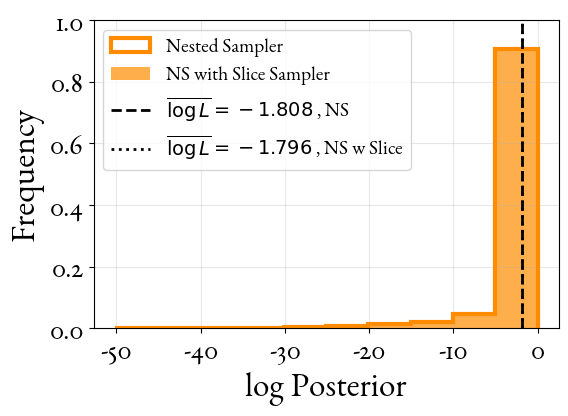
\includegraphics[width = 0.48\textwidth]{figures/MockFit/MockLogPost_Stel_3_lo.png}}\quad
  \subcaptionbox{Posterior for ISM dust }{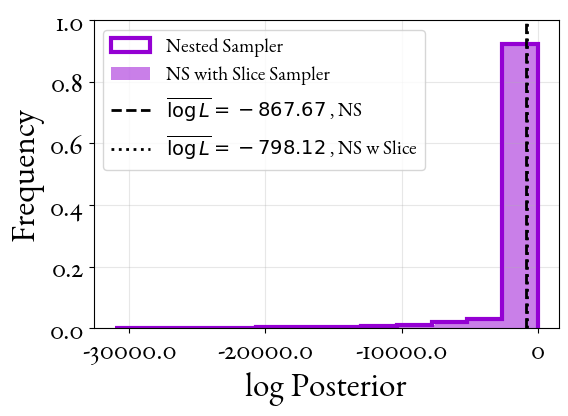
\includegraphics[width = 0.48\textwidth]{figures/MockFit/MockLogPost_Dust_3_lo.png}}\\
  \subcaptionbox{Posterior for BBB }{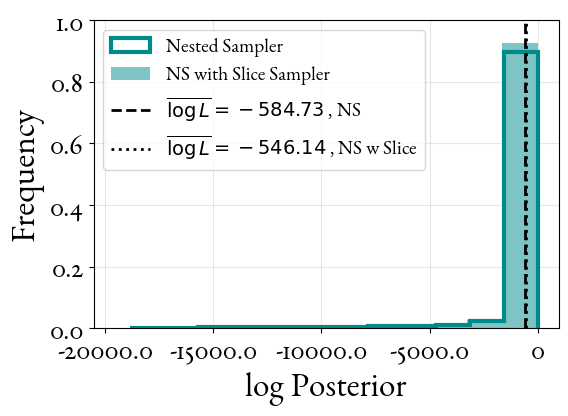
\includegraphics[width = 0.48\textwidth]{figures/MockFit/MockLogPost_BBB_3_lo.png}}\quad
  \subcaptionbox{Posterior for Torus}{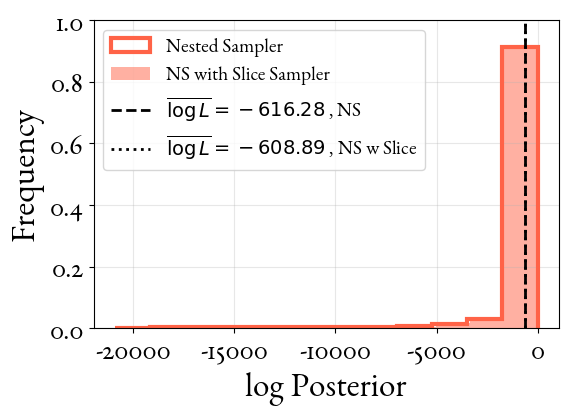
\includegraphics[width = 0.48\textwidth]{figures/MockFit/MockLogPost_Torus_3_lo.png}}\\

  \caption{Posterior distributions sampled by fitting a single component model to synthetic data from the same component. Panel (a): Stellar Population component posterior Panel (b): ISM dust component posterior. Panel (c): Accretion disk component posterior. Panel (d): AGN torus component posterior.}
  \label{fig:ComponentPosterior}
\end{figure}
\begin{figure}
  \subcaptionbox{Stellar Residuals }{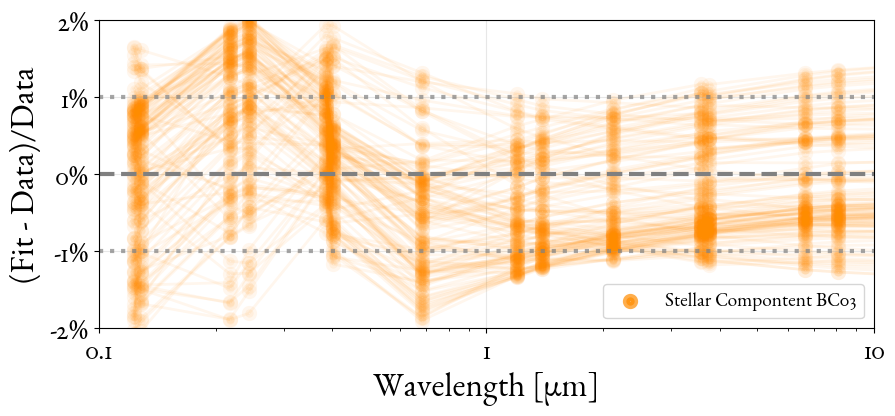
\includegraphics[width = 0.48\textwidth]{figures/MockFit/MockResid_Stel50_1_lo.png}}\quad
  \subcaptionbox{ISM dust Residuals }{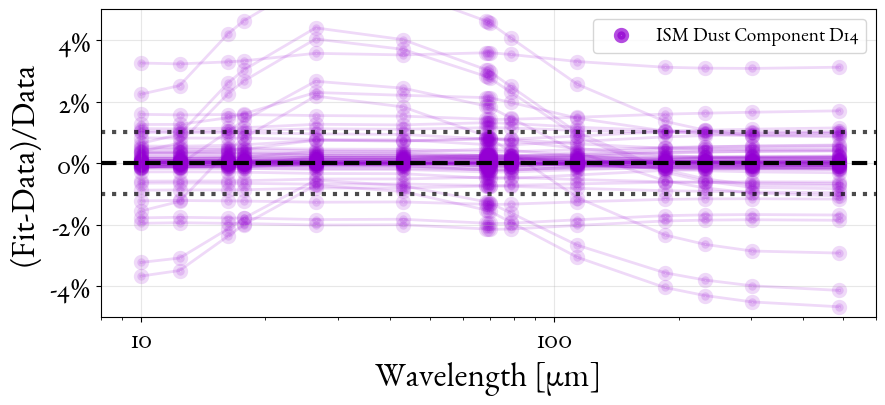
\includegraphics[width = 0.48\textwidth]{figures/MockFit/MockResid_Dust50_1_lo.png}}\\
  \subcaptionbox{BBB Residuals }{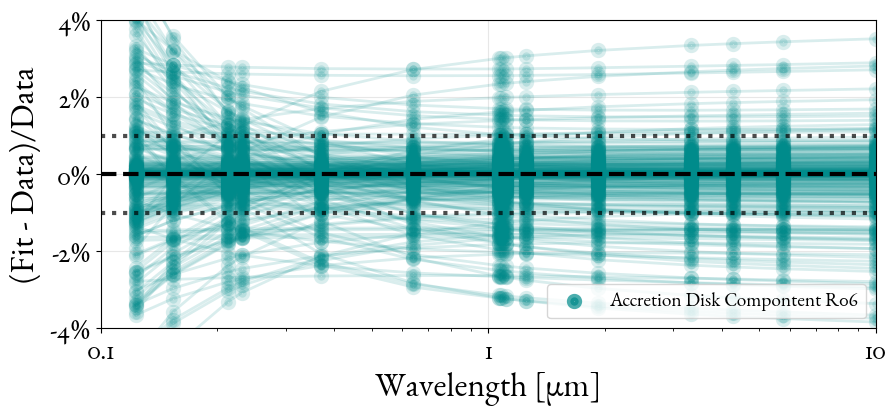
\includegraphics[width = 0.48\textwidth]{figures/MockFit/MockResid_BBB50_1c_lo.png}}\quad
  \subcaptionbox{Torus Residuals}{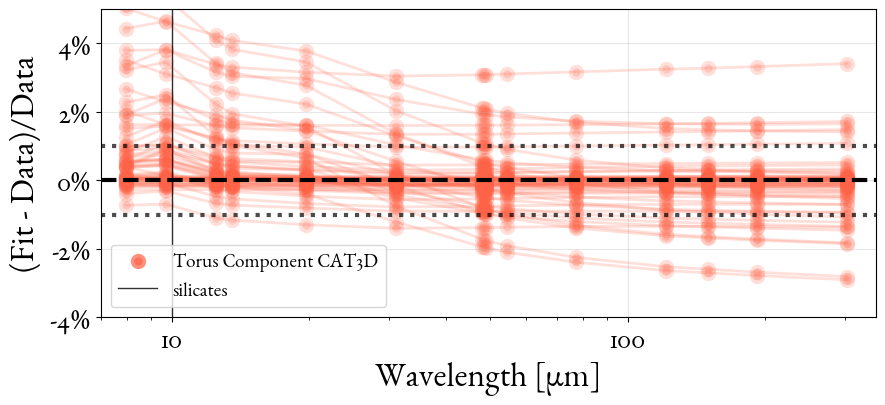
\includegraphics[width = 0.48\textwidth]{figures/MockFit/MockResid_Tor50_1_lo.png}}\\
  
  \caption{Component Residuals.}
  \label{fig:ComponentResiduals}
\end{figure}

\subsection*{Mock Galaxy Fits}
Mock galaxy SEDs are generated by intentionally combining model parametres with known physical properties and parametres, then adding Gaussian noise (in base-ten logarithmic scale). When fit with the algorithm, the posterior is plotted in Figure \ref{fig:MockSEDPost}, ascertaining the fit converged, 20 SEDs that correspond to the parametres of the 20 samples with the highest posterior value are plotted in Figure \ref{fig:MockSEDfit}, along with the synthetic data. The residuals indicate a remarkably high accuracy. 
\begin{figure}
\centering
  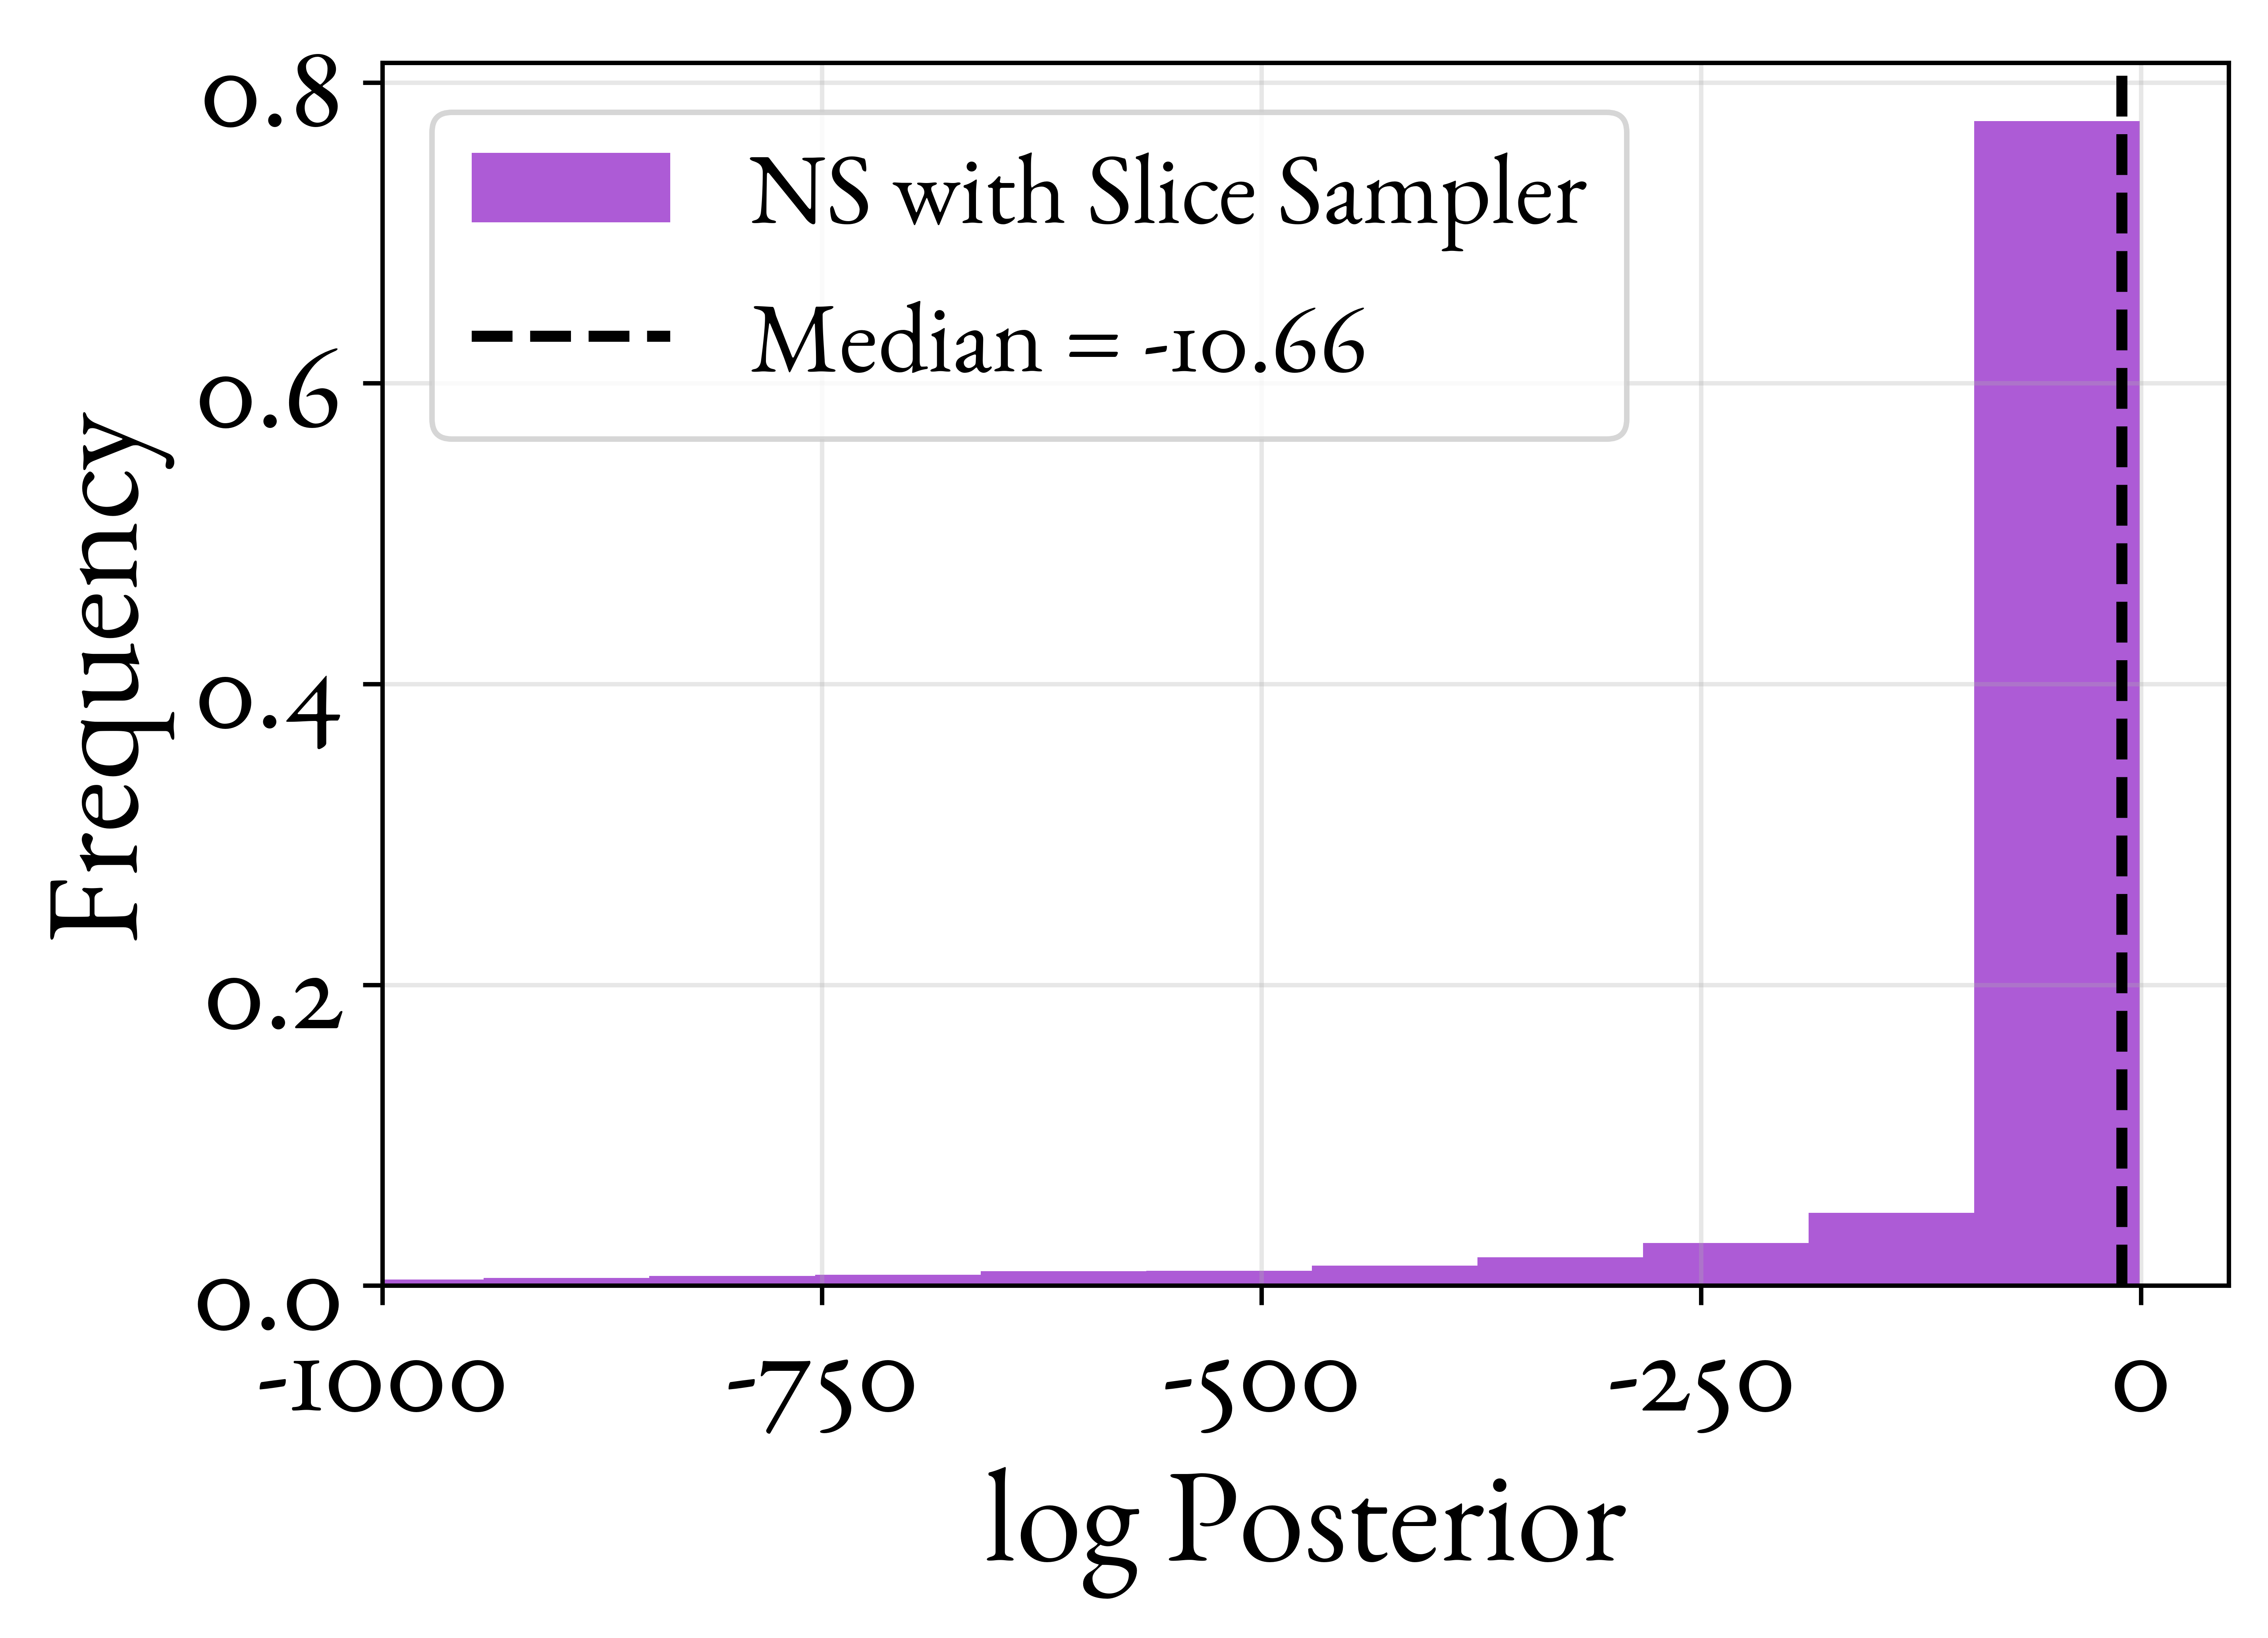
\includegraphics[width = 0.7\textwidth]{figures/MockFit/Mockfit_Posterior_1stel.png}
  \caption{Posterior distribution of a full SED fit of a Mock galaxy.}
  \label{fig:MockSEDPost}
\end{figure}

\begin{figure}
  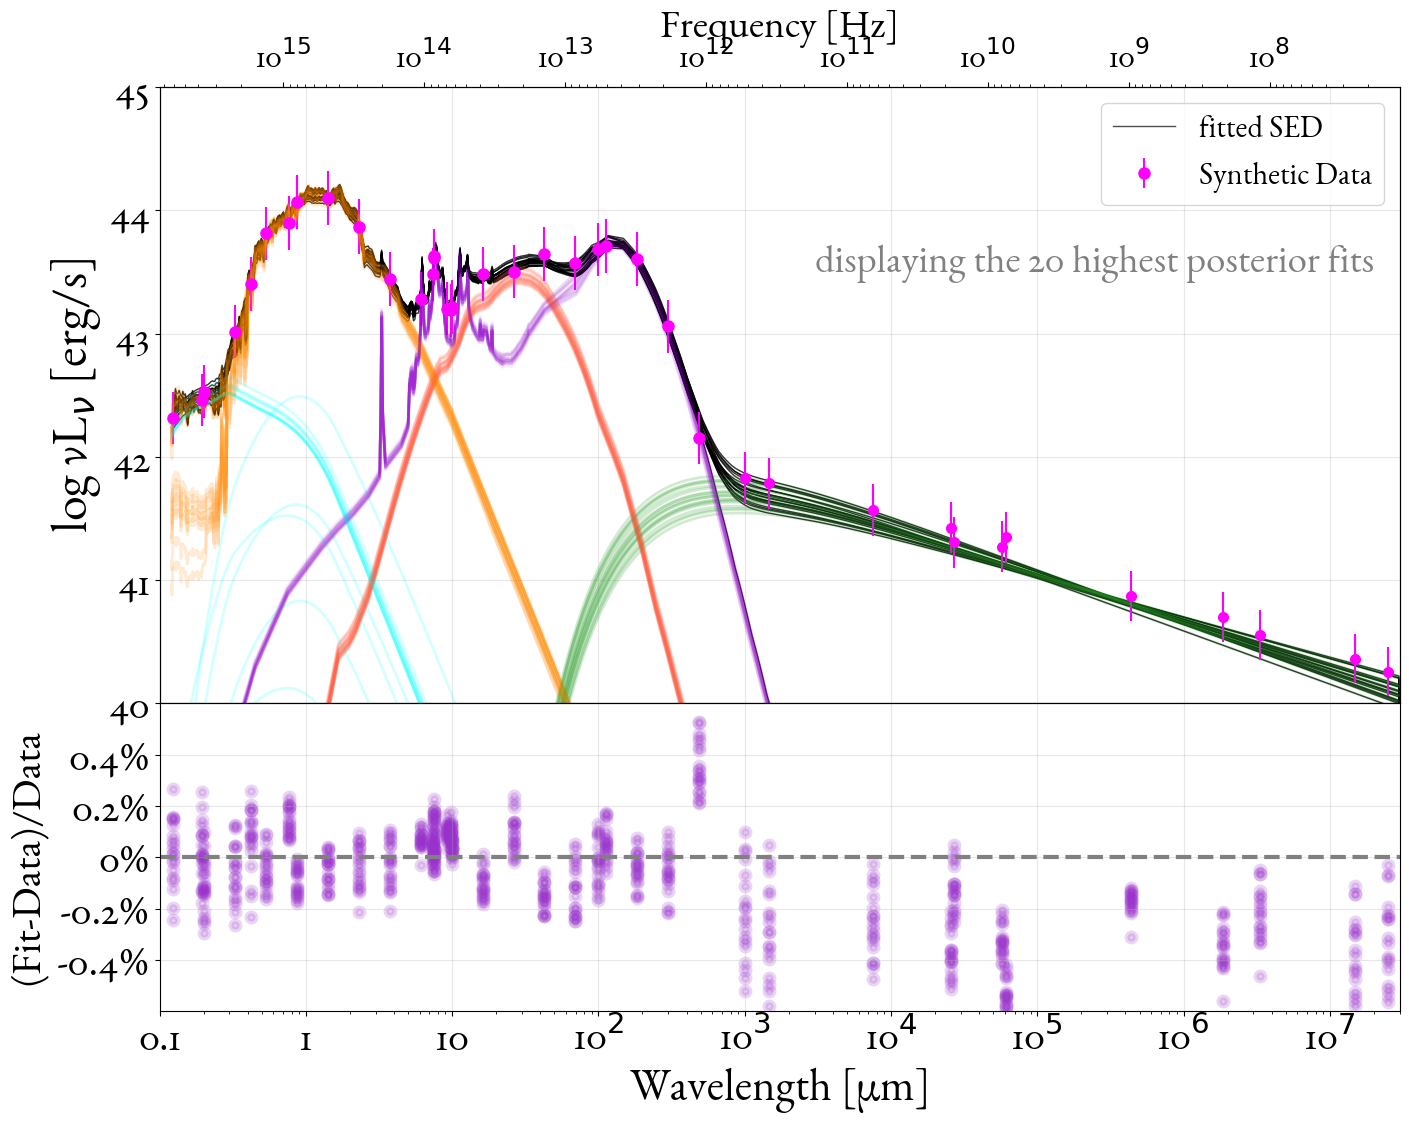
\includegraphics[width = \textwidth]{figures/MockFit/MockSEDfit_wRad_1stel_wPerCent_doubleaxes.png}
  \caption{SED model fit for synthetic data with logarithmic-Gaussian noise, representing a mock galaxy. The 20 highest posterior fits are plotted along with the synthetic data and each component is highlighted with color. }
  \label{fig:MockSEDfit}
\end{figure}

%---------------------------------------------------------------------------%
%---------------------------------------------------------------------------%
%---------------------------------------------------------------------------% 
\section{Fitting SED models to Data}

45 ARC galaxies are fit reliably using the code developed in this thesis. The most important factor impeding the algorithm to fit more galaxies is the absence of a blazar component, which can be improved in the future.\\ 
In Appendix \ref{app:Poster} each of the 45 ARC galaxies' mapped posterior distribution histogram is plotted in full scale and in the concentration region, verifying that each fit converged.\\
In Appendix \ref{app:MassDistri} each of the 45 ARC galaxies' sampled mass of young stellar population and old stellar population histograms are plotted clearly demarcating the median sampled value, the 16$^{\mbox{\tiny{th}}}$ and the 84$^{\mbox{\tiny{th}}}$ percentile of the sampled values, which are the credibility interval for the mass estimation. The masses are inferred in logarithmic scale, and the total inferred mass is $$ M_{\star, \mbox{\tiny{tot}} } = 10^{\mathcal{M}_{\star, \mbox{\tiny{old}} }} \; M_\odot + 10^{\mathcal{M}_{\star, \mbox{\tiny{young}} }} \; M_\odot$$ 
where 
\begin{equation*}
    \begin{cases}
        \mathcal{M}_{\star, \mbox{\tiny{old}} }= \log_{10} {M}_{\star, \mbox{\tiny{old}} }\\
        \mathcal{M}_{\star, \mbox{\tiny{young}} }= \log_{10} {M}_{\star, \mbox{\tiny{young}} }
    \end{cases}
\end{equation*}
In Appendix \ref{app:SEDFits} each of the 45 ARC galaxies' SED is plotted with 60 fit SED models which correspond to 60 randomly selected fits from the 10\% highest values of the sampled posterior distribution, along with the residuals, while the median total stellar mass inferred is denoted. Four indicative fit galaxies are shown in Figures \ref{fig:SEDfit} and \ref{fig:SEDfit2}.
All SEDs are portrayed in each galaxy's restframe. For most galaxies the fitted model is representative of the data, with the residuals in less than 2\%. 

\begin{figure}
    \centering
    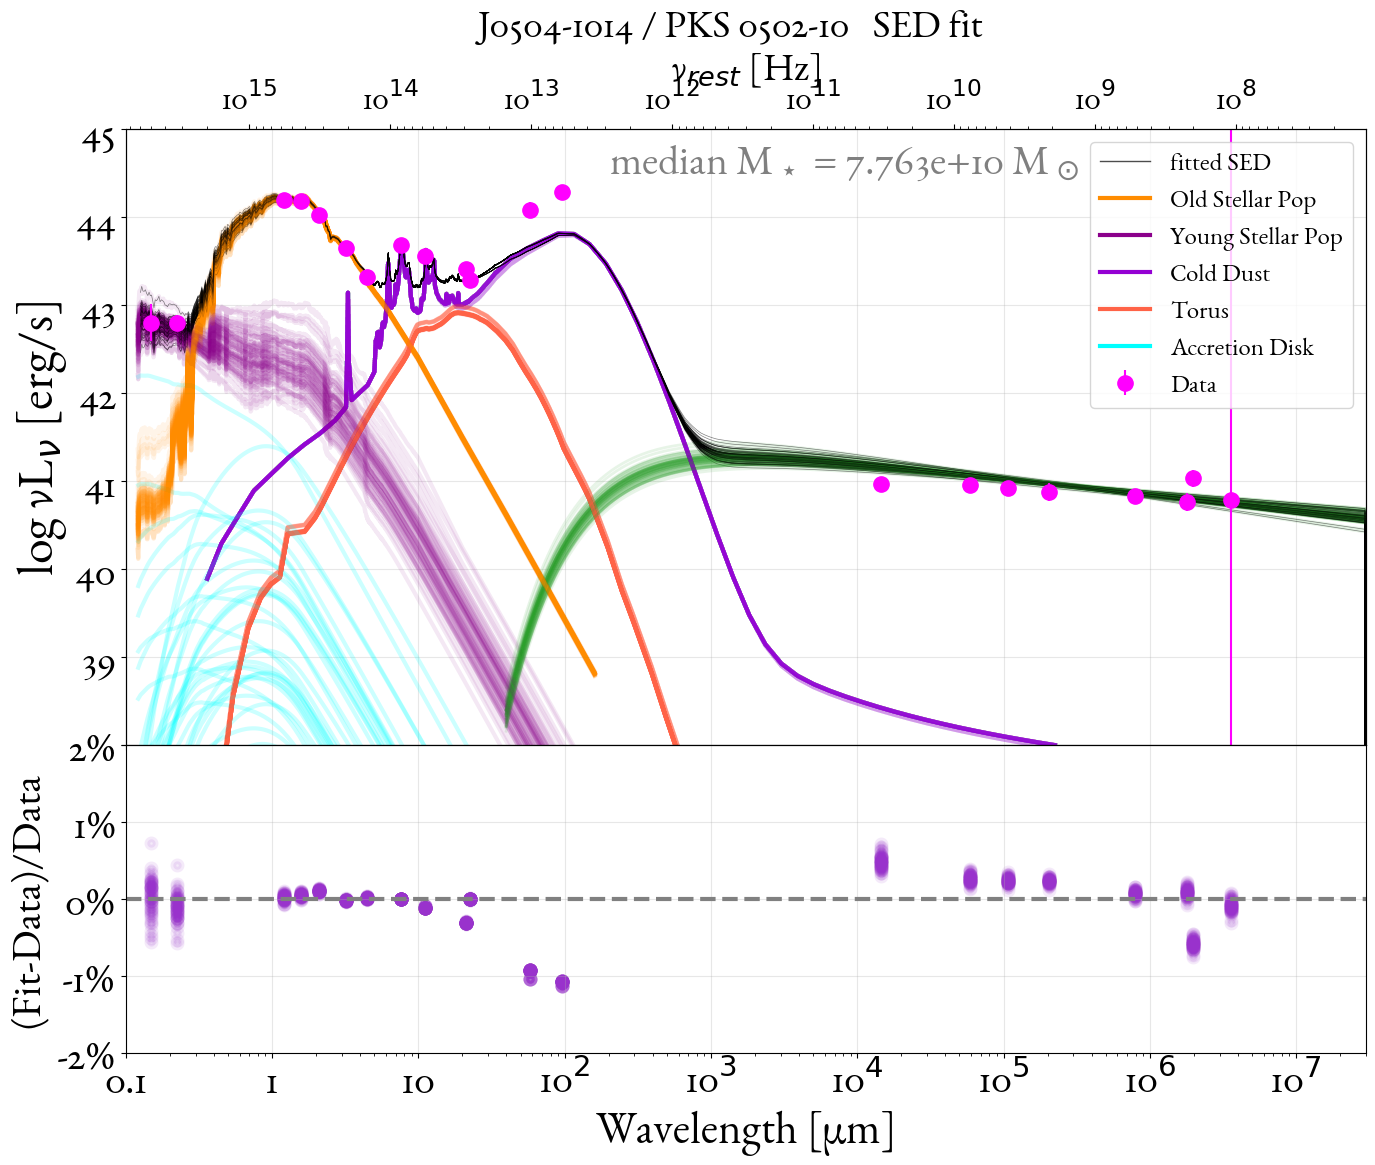
\includegraphics[width=0.75\linewidth]{figures/ResultFits/19_SEDfit_1765.png}\\
    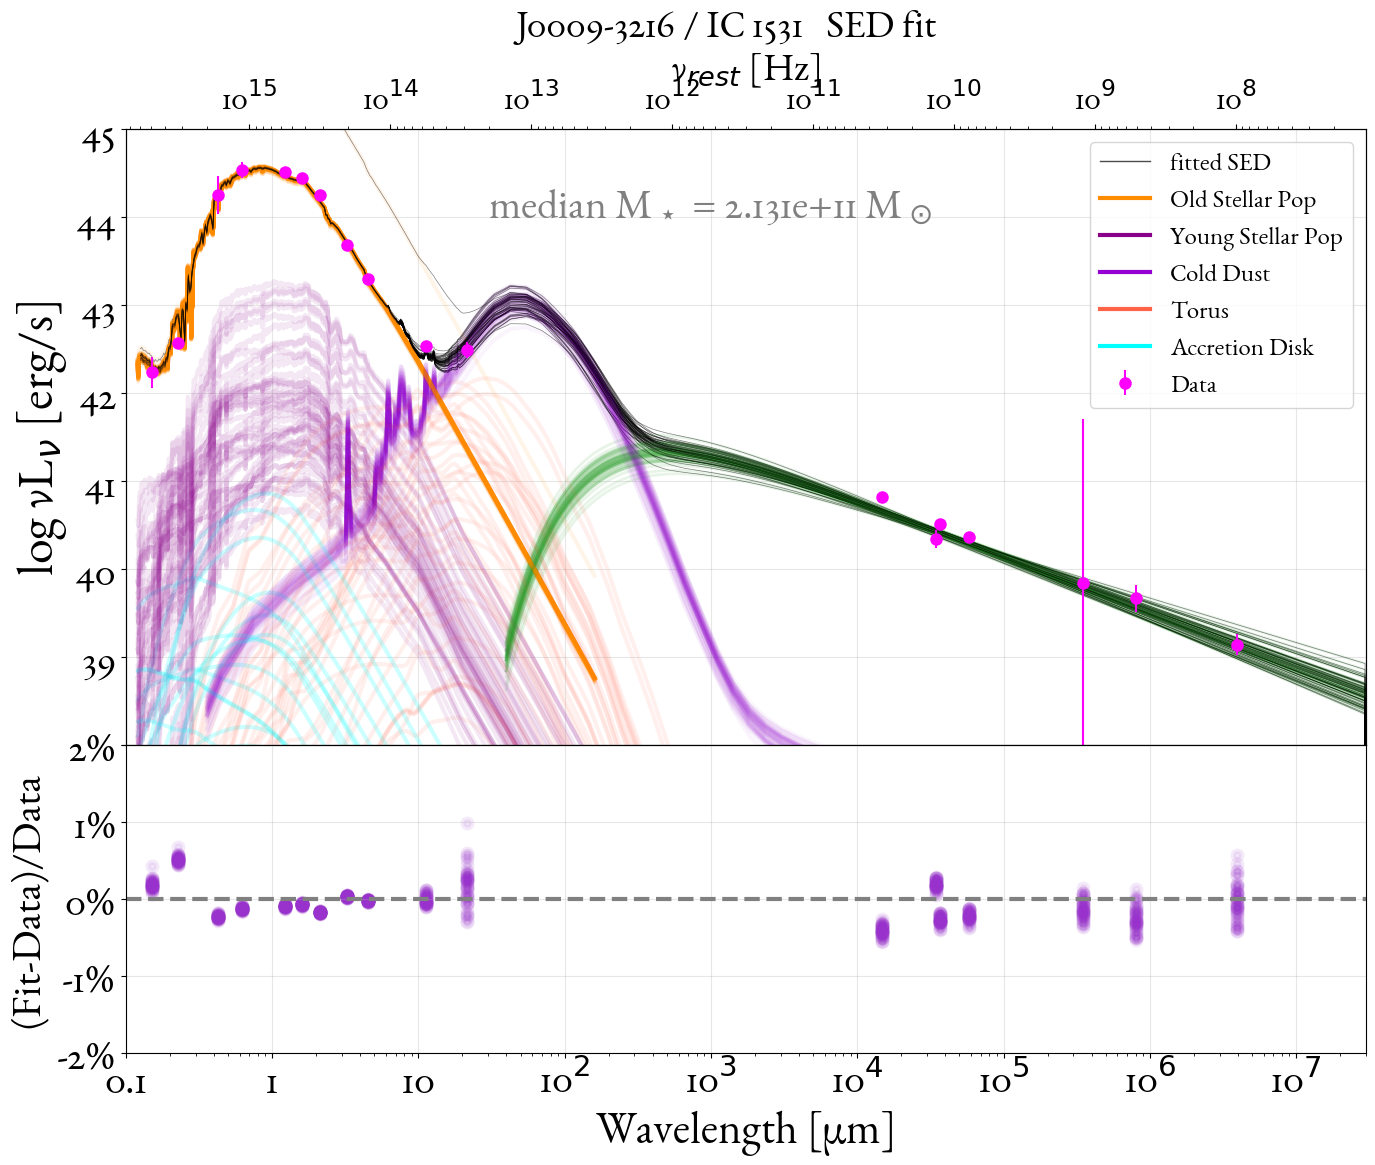
\includegraphics[width=0.75\linewidth]{figures/ResultFits/1_SEDfit_16.png} 
    \caption{SED fit for The ARC galaxies J0504-1014 and J0009-3216. Plots of the SED fit for all the 45 ARC sources can be found in Appendix \ref{app:SEDFits}. }
  \label{fig:SEDfit}
\end{figure}

\begin{figure}
    \centering
    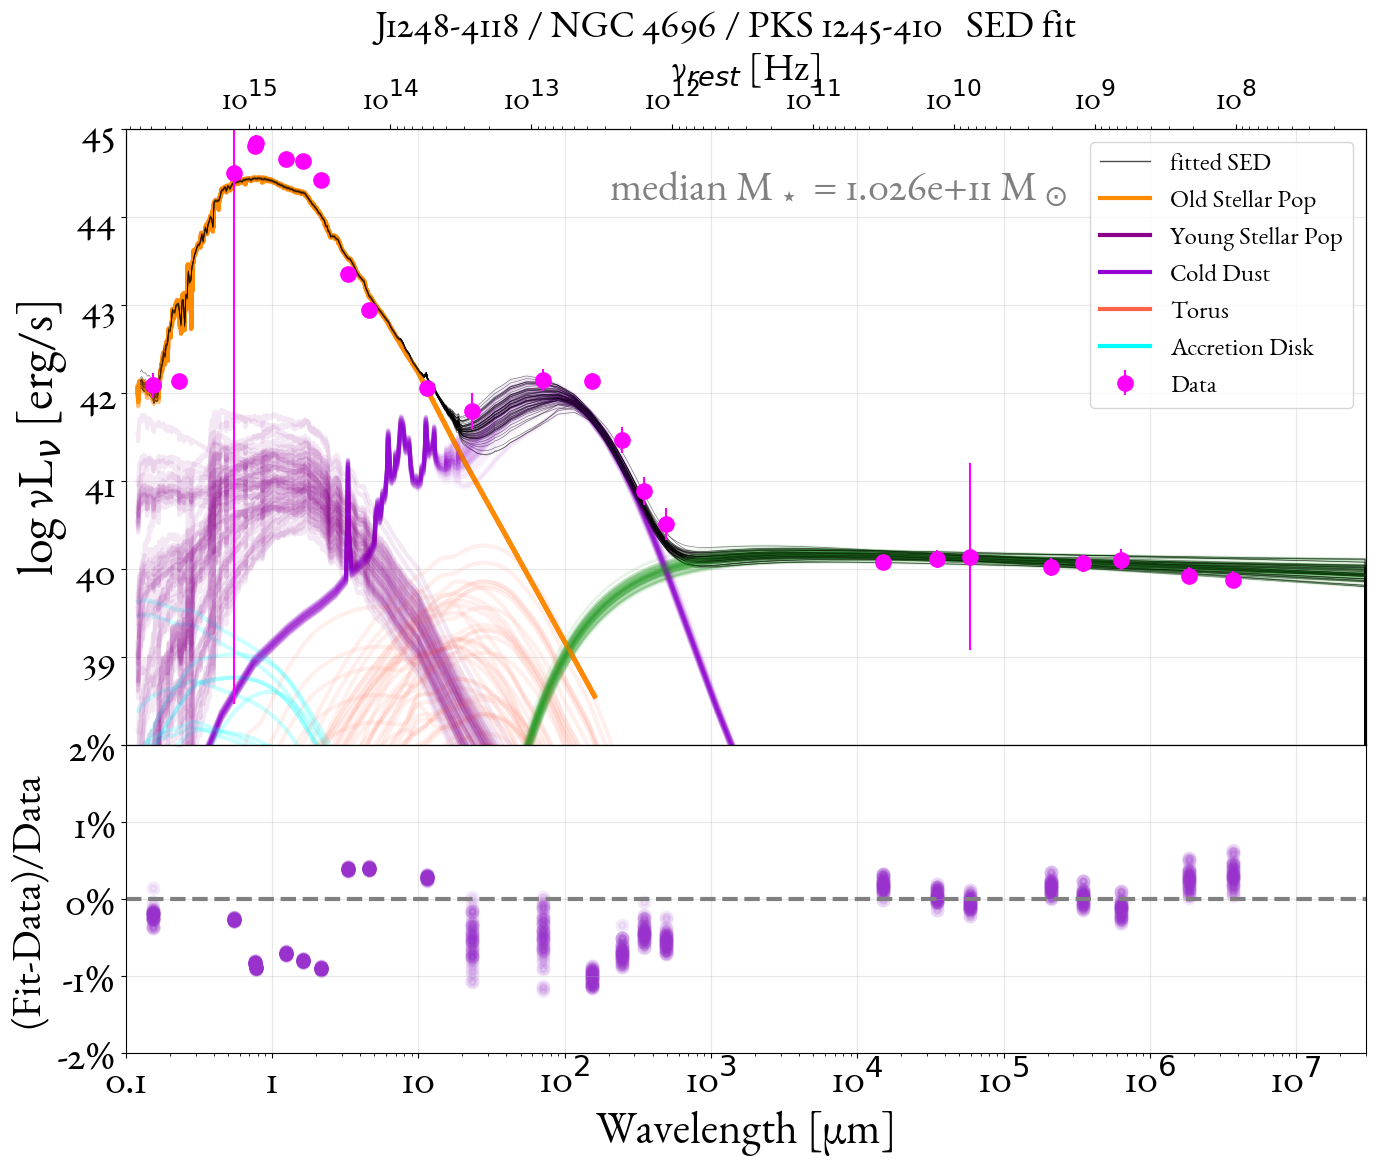
\includegraphics[width=0.75\linewidth]{figures/ResultFits/51_SEDfit_4126.png}\\
    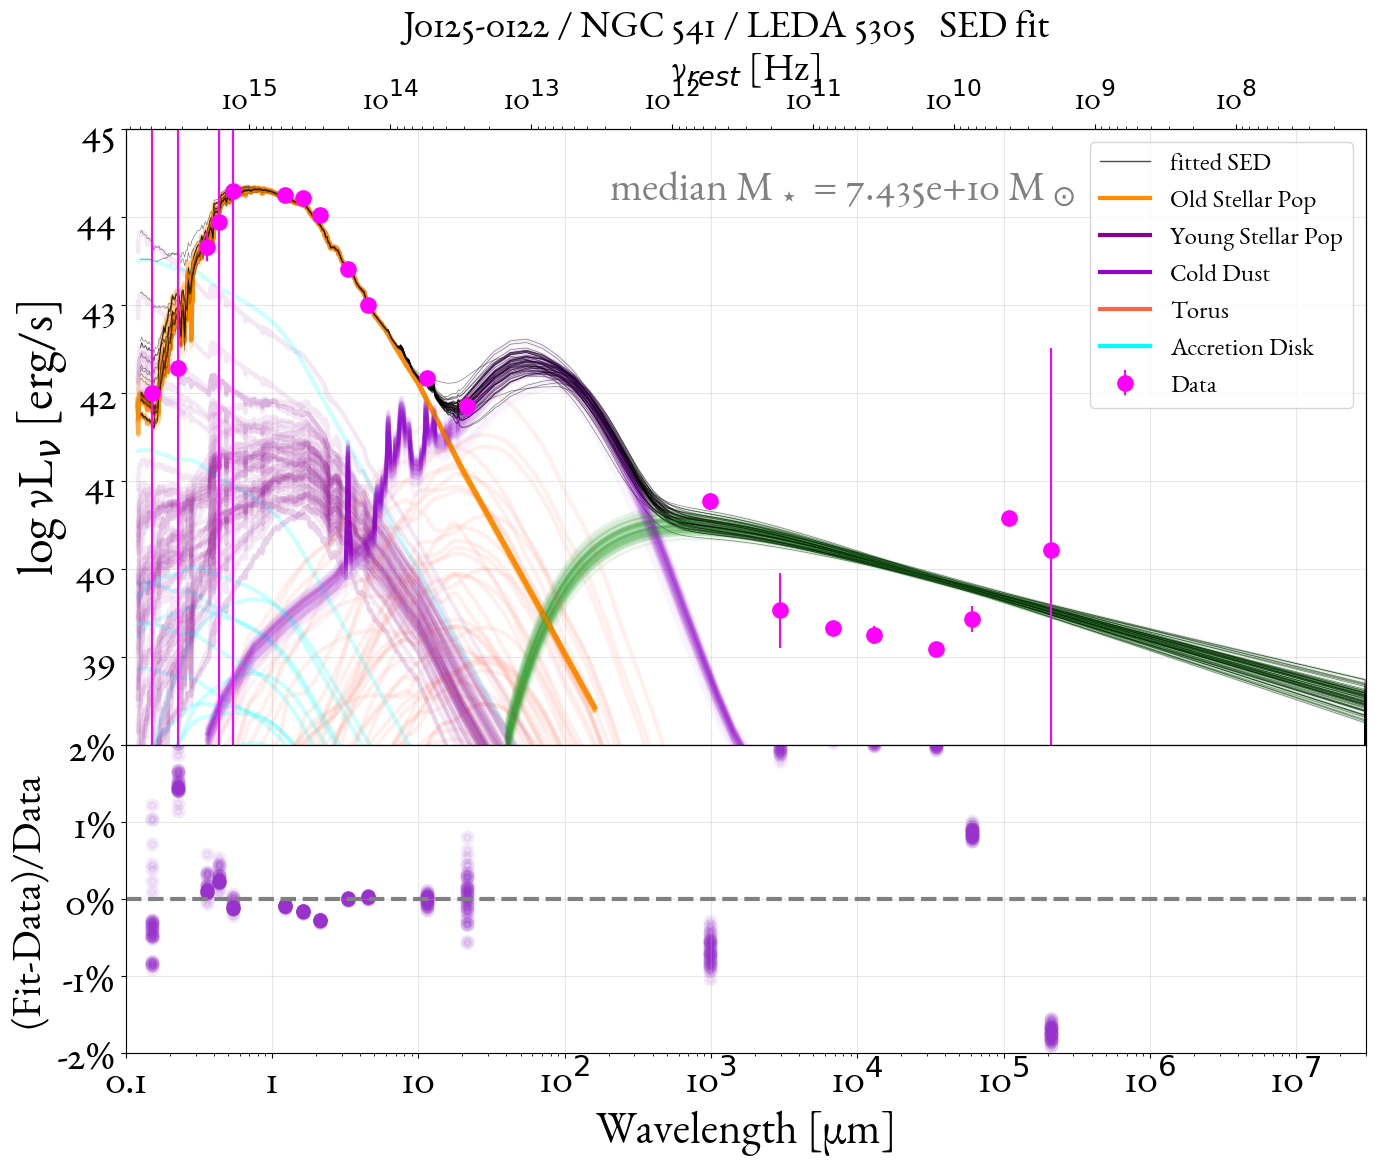
\includegraphics[width=0.75\linewidth]{figures/ResultFits/93_SEDfit_5260.png}
    \caption{SED fit for The ARC galaxies NGC 4696 and NGC 541. Plots of the SED fit for all the 45 ARC sources can be found in Appendix \ref{app:SEDFits}. }
  \label{fig:SEDfit2}
\end{figure}